\subsection{$d(K^-, n \pi^+ \pi^-)"n"$ final state identification and fine truning}
\begin{figure}[htbp]
  \centering
  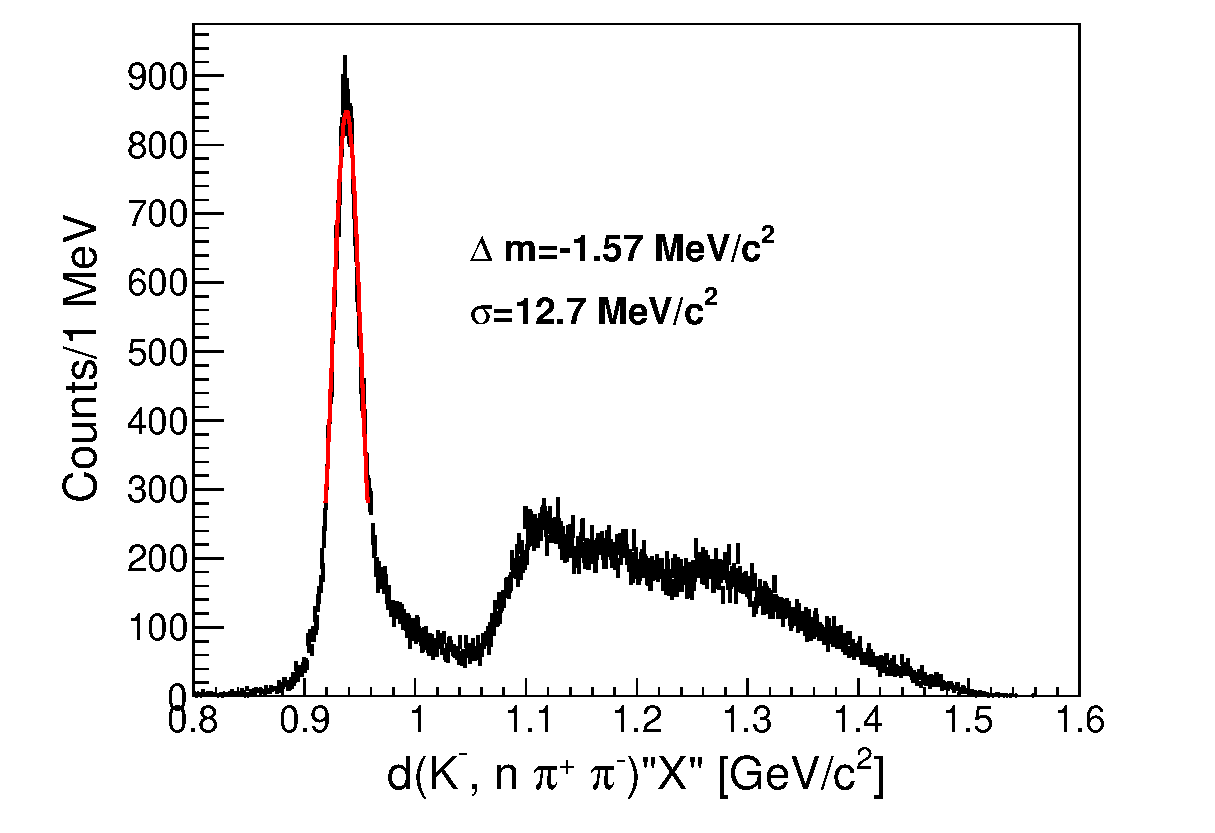
\includegraphics[width=10cm]{../pic/Run78/KN_ana/KNpipi_MM_woFit.eps}
  \caption{
    This figure shows $d(K^-, n \pi^+ \pi^-)"X"$ spectrum.
    Red line indicates fittig gaussian and gray hatched region indicates rejected region for $d(K^-, n \pi^+ \pi^-)"n"$ events.
  }
  \label{fig:KNpipi_MM}
\end{figure}

The $d(K^-, n)"\pi^{\mp}\Sigma^{\pm}"$ and the $d(K^-, n)"n K^0"$ mode were searched in the $d(K^-, n \pi^+ \pi^-)"n"$ final state.
Fig\ref{fig:KNpipi_MM} shows the missing mass of the $d(K^-, n \pi^+ \pi^-)$ in events detecting the forward neutron and the $\pi^{\pm}$ by the CDS.
These events was adopted the offline analysis selection to reject the accidental, which was described in Sec.\ref{sec:software_select_kn}. % To do add appendix

Although The time walk effect of the NC was calibrated using the $\gamma$ peak, the correlation was seen in the $d(K^-, n \pi^+ \pi^-)"n"$ peak as shown in the left figure of Fig\ref{fig:NC_recalib}.
The correlation was caused the difference of the $dE$ by the $\gamma$  and the neutron, which was seenFig\ref{fig:NC_beta}.

For this reason, we collected the momentum of the neutron following method.
The momenta of the $K^-$ beam, $\pi^-$, and $\pi^+$ was fixed and the momentum giving correct neutron mass was searched.
The correlation of the difference of momentum and the dE was collected by the 2nd-order-polynomial function as shown in Fig\ref{fig:NC_recalib}.

\begin{figure}[htbp]
  \begin{tabular}{cc}
    \begin{minipage}{0.5\hsize}
      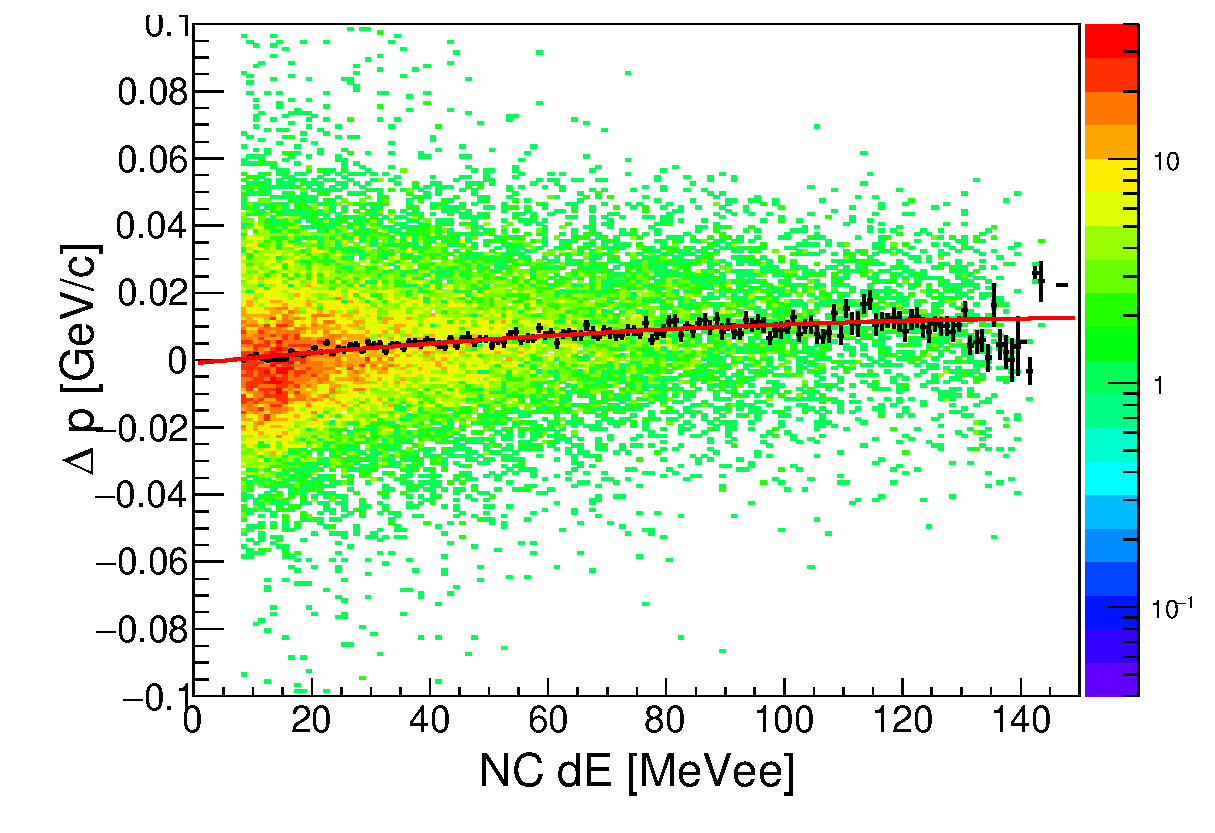
\includegraphics[width=5cm]{../pic/Run78/calib/NCdE_delta_p.eps}
    \end{minipage}
    \begin{minipage}{0.5\hsize}
      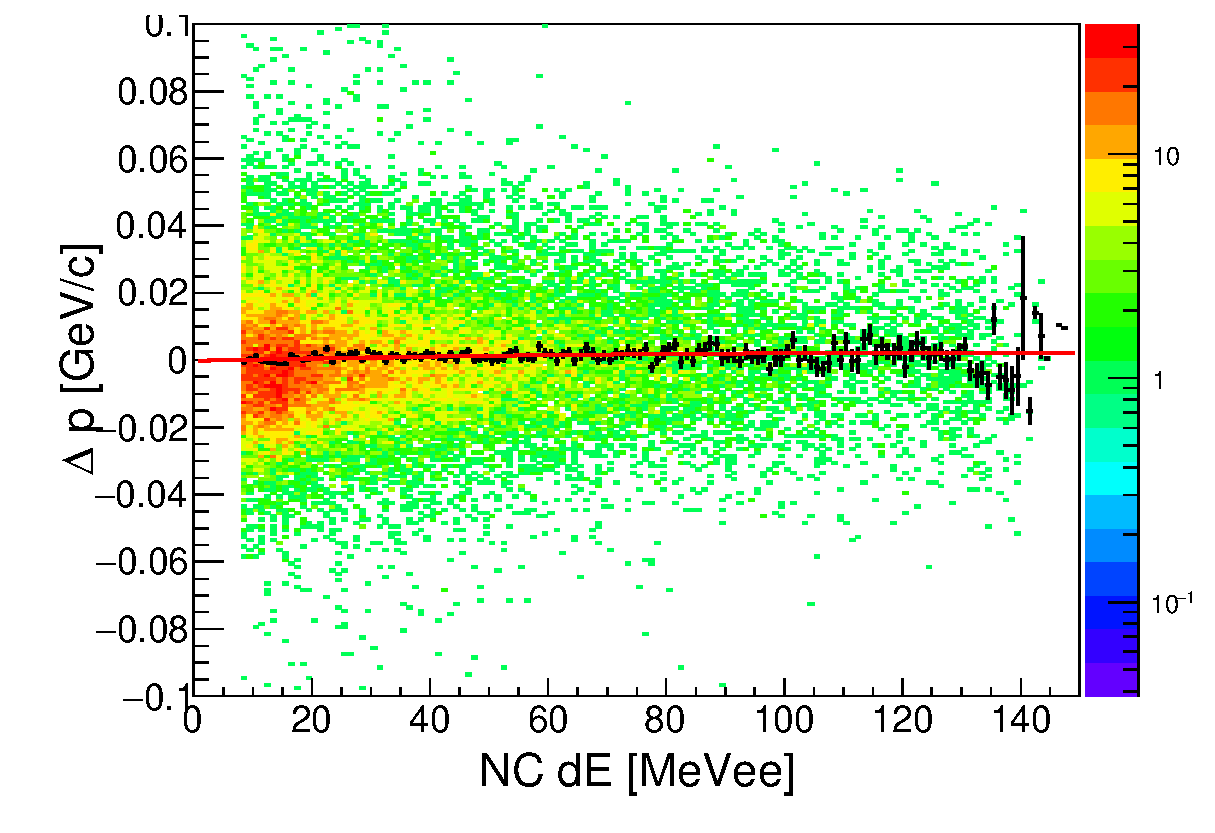
\includegraphics[width=5cm]{../pic/Run78/calib/NCdE_delta_p_mod.eps}
    \end{minipage}
  \end{tabular}
  \caption{
    These figures show $\Delta$ p which was calculated by given PDG value of neutron mass.
    Left figure represents before calibration and right figure represents after calibration.
  }
  \label{fig:NC_recalib}
\end{figure}

